\documentclass[11pt,a4paper]{article}
\usepackage[utf8]{inputenc}
\usepackage[T1]{fontenc}
\usepackage[brazilian]{babel}
\usepackage[margin=2.3cm]{geometry}
\usepackage{graphicx}
\usepackage{booktabs}
\usepackage{array}
\usepackage{xcolor}
\usepackage{hyperref}
\usepackage{caption}
\usepackage{subcaption}
\usepackage{amsmath}
\usepackage{longtable}
\usepackage{float}
\usepackage{enumitem}
\usepackage{multirow}
\usepackage{seqsplit}

\hypersetup{
  colorlinks=true,
  linkcolor=blue!50!black,
  urlcolor=blue!50!black,
  citecolor=blue!50!black
}

\title{CNN1D-Autoencoder para Detecção de Anomalias em Turbina\\
\large Migração de metodologia do AutoML, normalização restrita ao\\
período operacional e o candidato EXP15b}
\author{Pipeline \texttt{cnn1d\_ae} --- projeto \texttt{TesteMLCab} (Cabiunas/Petrobras)}
\date{Agosto de 2026}

\begin{document}
\maketitle

\begin{abstract}
Este relatório documenta a evolução do candidato de referência do
CNN1D-Autoencoder (CNN1D-AE) da série EXP13 para o novo candidato
\textbf{EXP15b}, motivada pela investigação de dois episódios reais não
detectados pelo candidato anterior (2026-03-25 e 2026-04-14). A
investigação separou as causas: o episódio de 2026-03-25 não era falha
do modelo (o autoencoder detectou, mas um portão de segurança bloqueou a
detecção por uma margem pequena demais para o mecanismo de resgate
existente); o de 2026-04-14 era uma falha real -- uma deriva lenta de
temperatura (+115°C em $\sim$24h) invisível ao modelo porque as
estatísticas de normalização eram contaminadas por $\sim$42\% de dados
de treino em período de parada/partida, comprimindo o sinal
padronizado de desvios reais dentro da operação. A correção
(\texttt{NORMALIZE\_ON\_STATE\_ONLY}, restringindo as estatísticas de
normalização ao período operacional) mais uma recalibração de
threshold guiada por regrid offline resultou no candidato
\textbf{EXP15b}: cobertura de alarme (\texttt{hit\_rate}) de
\textbf{77,5\% (31/40)}, superando o candidato anterior (75,0\%,
30/40), com falso alerta de \textbf{0,30\%} -- ainda bem abaixo do
melhor candidato AutoML de referência (0,35\%). Documentamos também a
origem híbrida da metodologia atual: boa parte dos mecanismos de
pós-processamento do CNN1D-AE (segundo critério da máscara operacional,
portão de rampa refinado, portão de volatilidade) foi \emph{herdada} de
uma série de experimentos AutoML (EXP7--EXP10) que investigou e reduziu
o falso alerta de um candidato \texttt{ocsvm} em $\sim$82\% relativo
antes de essas correções serem portadas de volta para o CNN1D-AE.
\end{abstract}

\tableofcontents

% =====================================================================
\section{Introdução e contexto}
% =====================================================================

O projeto \texttt{TesteMLCab} desenvolve detectores de anomalia para
sensores de uma turbina a gás da Cabiunas (Petrobras), com foco inicial
em temperatura de gás de escape (\texttt{TC382\_03\_A}/\texttt{T5\_AVG\_A})
e nos 10 canais de vibração de mancal associados. Duas famílias de
pipeline coexistem no repositório e compartilham infraestrutura de
avaliação:

\begin{itemize}[leftmargin=1.4em]
  \item \textbf{AutoML} (\texttt{src/cnn1d\_ae/automl\_pipeline.py}) ---
    modelos ponto-a-ponto (\texttt{dense}/\texttt{iforest}/\texttt{ocsvm})
    sobre um vetor de features por instante, sem janelamento temporal
    explícito no modelo. Testados numa grade ampla de hiperparâmetros
    (percentil de threshold, debounce) por sensor/grupo.
  \item \textbf{CNN1D-AE} (\texttt{src/cnn1d\_ae/pipeline.py}) --- o
    objeto deste relatório: um autoencoder convolucional 1-D que
    reconstrói janelas deslizantes multivariadas, buscado por
    KerasTuner e avaliado pelo erro de reconstrução (MAE).
\end{itemize}

As duas pipelines evoluíram em paralelo e, mais importante para este
relatório, \textbf{trocaram descobertas entre si}: mecanismos de
pós-processamento nascidos numa pipeline foram portados para a outra
sempre que uma investigação de falso positivo/falso negativo revelava
uma causa física que a outra pipeline também sofria. A Seção
\ref{sec:migracao} documenta essa migração em detalhe. A Seção
\ref{sec:metodologia} descreve a metodologia atual completa (dados,
janelas, split, arquitetura), incluindo a normalização restrita ao
período operacional -- a contribuição nova documentada aqui. A Seção
\ref{sec:resultados} apresenta os resultados comparativos, incluindo o
estudo de caso do episódio 2026-04-14 e a classificação dos 40 alarmes
do período de avaliação por qualidade de detecção. A Seção
\ref{sec:discussao} discute limitações, uma tentativa de mitigação
rejeitada (\texttt{THRESH\_MODE=target\_rate}) e pendências.

% =====================================================================
\section{Migração de metodologia: do AutoML para o CNN1D-AE}
\label{sec:migracao}
% =====================================================================

Nem toda melhoria no CNN1D-AE nasceu dentro dele. A série de
experimentos AutoML EXP5--EXP11 (\texttt{docs/analise\_automl\_exp*.md})
funcionou como um laboratório mais barato de iterar -- os modelos
ponto-a-ponto treinam em segundos a minutos contra horas do CNN1D-AE
-- e várias descobertas de lá foram portadas de volta. Esta seção
documenta essa migração na ordem em que aconteceu.

\subsection{Infraestrutura de avaliação compartilhada}

Antes de qualquer migração de \emph{mecanismo}, as duas pipelines já
compartilhavam a mesma régua de avaliação, definida em
\texttt{src/cnn1d\_ae/scoring.py} e usada por ambas:

\begin{itemize}[leftmargin=1.4em]
  \item \textbf{Split out-of-sample (OOS) temporal}: o modelo (e, no
    CNN1D-AE, a normalização e o threshold) só enxerga dados anteriores
    a \texttt{OOS\_SPLIT\_DATE}; a avaliação de \texttt{hit\_rate}/
    \texttt{normal\_alert\_rate} só considera alarmes e pontos
    posteriores ao corte. A escolha do corte não é arbitrária --
    EXP5 (AutoML) documentou um achado negativo em que mover o corte
    OOS sem checar a distribuição de alarmes destruiu o poder
    estatístico da avaliação (a amostra de alarmes na fatia de teste
    caiu de 70 para 4--8).
  \item \textbf{\texttt{eval\_alarm\_hit\_rate}}: para cada alarme real
    do catálogo, verifica se existe algum ponto marcado como anômalo
    numa janela de $\pm$\texttt{EXCLUDE\_MINUTES\_AROUND\_ALARM}
    (24h) ao redor do timestamp do alarme.
  \item \textbf{\texttt{compute\_composite\_score}}: combina
    \texttt{hit\_rate} e \texttt{normal\_alert\_rate} (falso alerta) num
    único escore, penalizando falso alerta quadraticamente -- usado
    para ranquear candidatos/trials.
  \item \textbf{Seed-sweep}: re-treina a mesma arquitetura vencedora com
    N sementes extras e reporta a variação de \texttt{hit\_rate}/
    \texttt{normal\_alert\_rate}. Nasceu no AutoML (EXP5,
    \texttt{AUTOML\_SEED\_SWEEP\_N}, motivado por uma variância de
    $\sim$27pp observada num autoencoder \texttt{dense} anterior) e foi
    portado para o CNN1D-AE, onde revelou o mesmo problema em escala
    menor (Seção~\ref{sec:seedsweep}).
\end{itemize}

Essa infraestrutura compartilhada é o que torna a comparação
AutoML~$\leftrightarrow$~CNN1D-AE do restante deste relatório
legítima: ambos são avaliados pela mesma função sobre o mesmo conjunto
de 40 alarmes OOS de \texttt{TC382\_03\_A}/\texttt{T5\_AVG\_A}.

\subsection{Features multiescala e de textura (herdado do AutoML EXP7)}
\label{sec:multiescala}

O EXP7 (AutoML) introduziu features derivadas em múltiplas escalas de
tempo -- média/desvio móvel e tendência (\texttt{roll\_med}/
\texttt{roll\_std}/\texttt{trend}) nas janelas de 6\,min, 1\,h, 4\,h e
24\,h (\texttt{DERIVED\_ROLLING\_WINDOWS = [12, 120, 480, 2880]}
amostras a 30\,s) -- e, para janelas $\geq$60 amostras, features de
``textura'' do sinal (\emph{kurtosis}, \emph{skewness}, \emph{crest
factor} = pico/RMS), comuns em \emph{condition monitoring} de vibração
para capturar um sinal ficando mais ``impulsivo'' antes de uma falha de
mancal. O ganho reportado no AutoML foi limpo e sem custo adicional de
falso alerta. O mesmo bloco de código (\texttt{\_build\_derived\_features},
\texttt{preprocess.py}) e os mesmos parâmetros de janela são usados,
sem alteração, no CNN1D-AE -- é a mesma implementação compartilhada
entre as duas pipelines, não uma reimplementação.

\subsection{Máscara operacional: segundo critério (herdado do AutoML EXP10)}
\label{sec:mascara-migracao}

O EXP10 (AutoML) fragmentou a série de falso alerta em episódios
contínuos e cruzou cada um com o dado bruto e o catálogo completo de 47
tags de alarme (não só os 2 sensores avaliados). Achado: 65,3\% do
falso alerta positivo (OOS) vinha de um único desligamento real de 3,5
dias em que \texttt{TC382\_03\_A} caía de $\sim$478°C para
$\sim$28--32°C enquanto \texttt{RUNNING\_A} (referência da máscara
operacional) permanecia em $\sim$0,96--1,0 o tempo todo -- a máscara
nunca reconhecia esse período como ``desligado''. A correção:
\texttt{build\_operational\_state} (\texttt{scoring.py}) ganhou um
segundo critério de ``off'', baseado no próprio sensor-alvo do grupo
caindo abaixo de um piso físico
(\texttt{secondary\_series}/\texttt{secondary\_off\_abs\_threshold}, ou
\texttt{OFF\_TARGET\_ABS\_THRESHOLD} na config), unido por OR ao
critério de \texttt{OPERATIONAL\_REF\_SENSOR} antes da classificação
\texttt{off\_curto}/\texttt{off\_longo}/\texttt{transiente}. Redução de
FP no AutoML: 1,94\%$\to$0,67\%, \texttt{hit\_rate} idêntico (92,5\%).
Essa mesma função é usada pelo CNN1D-AE (config atual:
\texttt{OFF\_TARGET\_ABS\_THRESHOLD=150,0°C}).

\subsection{Portão de rampa: originou no CNN1D-AE, refinado no AutoML (EXP10b)}

Diferente dos demais mecanismos desta seção, o portão de rampa
(\texttt{ENABLE\_LOAD\_GATE}/\texttt{apply\_load\_gate}) \textbf{já
existia no CNN1D-AE antes} e nunca havia sido portado para o AutoML.
O EXP10b portou-o, mas os parâmetros \emph{default} do CNN1D-AE
(\emph{halflife}=120\,min/janela=360\,min) custavam até 6 detecções
preditivas genuínas no AutoML -- uma rampa de falha real e uma manobra
de carga legítima têm a mesma assinatura de taxa de variação numa
janela longa. Uma janela mais curta
(\emph{halflife}=15\,min/janela=30\,min) + \texttt{ramp\_max=100°C/h},
encontrados por simulação offline sobre os dados reais do AutoML,
preservaram 29/29 detecções preditivas com FP caindo de 0,67\% para
0,48\%. Esse achado de janela-curta-preserva-preditivos informou a
recalibração do próprio portão de rampa do CNN1D-AE em rodadas
posteriores do EXP13 (ver \texttt{docs/analise\_cnn1dae\_exp13.md}) --
uma migração de \emph{ida e volta} entre as duas pipelines.

\subsection{Portão de volatilidade: nascido no AutoML, portado para o CNN1D-AE (EXP10c)}
\label{sec:volgate-migracao}

O portão de rampa reage a variação de \emph{nível}, mas o padrão de
falso alerta residual do EXP10b era diferente: o desvio-padrão dos
canais de vibração subia e \textbf{permanecia} elevado por 1--2h -- não
um pico de subida, mas uma volatilidade persistente. A primeira
tentativa (alimentar o portão de rampa existente com um índice de
volatilidade de vibração no lugar do proxy de temperatura, mantendo o
mecanismo de \emph{taxa de variação}) falhou: reduzia o FP de 0,480\%
para apenas 0,477\% -- taxa de variação não distingue o início de uma
rampa real do início de uma escalada de falha, o mesmo problema do
portão de rampa original, agora por métrica errada em vez de janela
errada. A segunda tentativa funcionou e é um mecanismo genuinamente
\textbf{novo}, sem equivalente prévio em nenhuma das duas pipelines:
\texttt{compute\_volatility\_index}/\texttt{apply\_volatility\_gate}
(\texttt{scoring.py}) -- desvio-padrão móvel causal de cada canal de
vibração, reduzido pela média entre canais, bloqueando quando o
\textbf{nível} (não a taxa) ultrapassa um threshold. Simulação offline
encontrou o ponto de custo zero: FP caindo mais 27\% relativo
(0,48\%$\to$0,35\%), preservando as 29/29 detecções preditivas. Esse
mecanismo -- inteiramente uma descoberta do AutoML -- foi portado para
o CNN1D-AE no EXP13 (commit \texttt{542d203}, ``port dos gates EXP10
pro CNN1D-AE'') e é hoje um dos quatro portões da camada de
pós-processamento descrita na Seção~\ref{sec:arquitetura}.

\subsection{Resumo da migração}

\begin{table}[H]
\centering
\small
\begin{tabular}{@{}p{4.1cm}p{3.4cm}p{5.7cm}@{}}
\toprule
\textbf{Mecanismo} & \textbf{Origem} & \textbf{Direção da migração} \\
\midrule
Split OOS temporal, \texttt{eval\_alarm\_hit\_rate}, \texttt{composite\_score} & Compartilhado desde o início & Infraestrutura comum (\texttt{scoring.py}) \\
Seed-sweep & AutoML (EXP5) & AutoML $\to$ CNN1D-AE \\
Features multiescala + textura & AutoML (EXP7) & AutoML $\to$ CNN1D-AE (mesma implementação) \\
2º critério da máscara operacional & AutoML (EXP10) & AutoML $\to$ CNN1D-AE \\
Portão de rampa (parâmetros refinados) & CNN1D-AE (original) $\to$ AutoML (EXP10b) & CNN1D-AE $\to$ AutoML $\to$ CNN1D-AE (recalibração) \\
Portão de volatilidade & AutoML (EXP10c) & AutoML $\to$ CNN1D-AE (EXP13) \\
Bloqueio gradual (\emph{gate-escape}) & CNN1D-AE (EXP13) & Original, sem equivalente no AutoML \\
Normalização restrita ao período operacional & CNN1D-AE (este relatório, EXP15b) & Original, sem equivalente no AutoML \\
\bottomrule
\end{tabular}
\caption{Origem e direção de migração de cada mecanismo da pipeline atual.}
\end{table}

% =====================================================================
\section{Metodologia}
\label{sec:metodologia}
% =====================================================================

\subsection{Dados}

\begin{itemize}[leftmargin=1.4em]
  \item \textbf{Fonte}: \texttt{sensores\_full\_2024\_2026\_30s.csv} --
    12 canais a 30\,s de resolução: \texttt{TC382\_03\_A} (alvo),
    \texttt{T5\_AVG\_A} (referência de carga) e 10 canais de vibração
    de mancal (\texttt{TV\_35\{1..5\}\{X,Y\}\_A}).
  \item \textbf{Período}: \texttt{DATA\_START\_DATE=2024-07-01} até o
    fim da série disponível ($\sim$abril de 2026).
  \item \textbf{Alarmes}: \texttt{alarmes\_selecionados\_turbina\_a.csv}
    -- catálogo de alarmes do SCADA. A avaliação usa só eventos de
    ativação (\texttt{Status} iniciando em \texttt{ACT}, excluindo
    pares de recuperação \texttt{INACT}) dos sensores \texttt{TC382\_03\_A}/
    \texttt{T5\_AVG\_A}, no período OOS: \textbf{40 alarmes}.
  \item \textbf{Split OOS}: \texttt{OOS\_SPLIT\_DATE=2025-07-01} --
    treino (modelo + normalização + threshold) só vê dados anteriores;
    avaliação só considera alarmes/pontos posteriores.
\end{itemize}

\subsection{Pré-processamento e janelas}

O pipeline segue sete fases, documentadas em detalhe em
\texttt{docs/preprocessamento\_entrada\_modelo.md} e resumidas na
Figura~\ref{fig:pipeline}:

\begin{enumerate}[leftmargin=1.4em]
  \item \textbf{Carregamento e normalização temporal} -- parsing de
    timestamp, conversão para UTC naive.
  \item \textbf{Construção do dataframe do grupo} -- alinhamento dos 12
    sensores no mesmo índice, interpolação de lacunas curtas
    ($\leq$3 amostras), máscara de gaps longos (OR entre sensores).
  \item \textbf{Máscara de exclusão de alarme} -- janela bilateral de
    $\pm$24h ao redor de cada alarme excluída do treino
    (\texttt{EXCLUDE\_MINUTES\_AROUND\_ALARM=1440}).
  \item \textbf{Clipping de outliers} -- modo \texttt{quantile}
    (percentis 0,1\%/99,9\%), limites calculados só sobre dados de
    treino.
  \item \textbf{Normalização treino-apenas} -- z-score (média/desvio),
    estatísticas calculadas exclusivamente sobre dados sem alarme e sem
    gap longo. \textbf{Contribuição nova deste relatório}: restrição
    adicional ao período operacional, Seção~\ref{sec:normalizacao-on-state}.
  \item \textbf{Sequências deslizantes} -- janelas de
    \texttt{TIME\_STEPS=60} amostras (30\,min a 30\,s/amostra) com
    \texttt{STRIDE=15} (7,5\,min entre janelas consecutivas) --
    tensor $(N, 60, 12)$.
  \item \textbf{Split treino/validação} -- temporal, 90\%/10\%
    (\texttt{VAL\_FRAC=0,1}), sem embaralhar (evita vazamento entre
    janelas sobrepostas).
\end{enumerate}

O princípio central, preservado em todas as versões da pipeline: as
estatísticas de pré-processamento (clipping, normalização, threshold)
são calculadas exclusivamente sobre dados normais, mas a
\textbf{inferência roda sobre a série completa}, incluindo períodos
anômalos -- é essa assimetria que faz uma anomalia elevar o erro de
reconstrução.

\subsection{Arquitetura e treino do autoencoder}
\label{sec:arquitetura}

O CNN1D-AE (\texttt{src/cnn1d\_ae/model.py}) é buscado por KerasTuner
(\texttt{RandomSearch}, \texttt{MAX\_TRIALS=40}) sobre o espaço:

\begin{center}
\small
\begin{tabular}{@{}ll@{}}
\toprule
Hiperparâmetro & Espaço de busca \\
\midrule
filtros da 1ª/2ª camada conv. & $\{8, 16, 32, 64\}$ \\
tamanho de kernel 1ª/2ª camada & $\{3, 5, 7, 9\}$ \\
\emph{dropout} & $[0{,}0, 0{,}4]$, passo $0{,}1$ \\
taxa de aprendizado & $\{10^{-4}, 3{\times}10^{-4}, 10^{-3}, 3{\times}10^{-3}\}$ \\
\emph{stride} 1ª/2ª camada conv. & $\{1, 2\}$ \\
\bottomrule
\end{tabular}
\end{center}

Arquitetura (encoder--decoder simétrico, ativação ReLU, saída linear):

\begin{multline*}
\text{Conv1D}(f_1,k_1,s_1) \to \text{Dropout} \to \text{Conv1D}(f_2,k_2,s_2)
\to \text{Conv1DTranspose}(f_2,k_2,s_2) \\
\to \text{Dropout} \to
\text{Conv1DTranspose}(f_1,k_1,s_1) \to \text{Conv1DTranspose}(12,3)
\end{multline*}

Otimizador Adam, perda MSE, \texttt{EarlyStopping} (\texttt{patience=5},
\texttt{restore\_best\_weights=True}) + \texttt{ReduceLROnPlateau}.
Tanto o candidato anterior (task 14) quanto o EXP15b convergiram para a
\textbf{mesma arquitetura vencedora} (seed principal 42, mesmo espaço
de busca): $f_1{=}64$, $f_2{=}32$, $k_1{=}k_2{=}7$, \emph{dropout}$=0$,
$lr{=}3{\times}10^{-4}$, $s_1{=}s_2{=}1$ -- a diferença de resultado
entre os dois candidatos vem inteiramente da normalização de entrada e
da recalibração do threshold, não de uma arquitetura diferente.

O erro de reconstrução é o MAE médio no eixo temporal, por sequência e
por canal (\texttt{reconstruction\_mae\_per\_seq}); quando o grupo
define um \texttt{target\_sensor} (aqui, \texttt{TC382\_03\_A}), o
threshold e a detecção usam só o MAE desse canal, não a média entre os
12 canais do grupo -- os demais canais entram como \emph{features} de
contexto para o autoencoder, não como alvo de detecção.

\subsection{Threshold e mapeamento sequência$\to$ponto}

O threshold usa o modo \texttt{robust\_mad}: mediana + $K \times
1{,}4826 \times \text{MAD}$ do MAE de treino -- robusto a caudas longas
que fariam \texttt{mean\_std} produzir um limiar inatingível. Sequências
com MAE acima do threshold são mapeadas para pontos via
\texttt{POINT\_RULE=k\_of\_window} (\texttt{POINT\_WINDOW=2},
\texttt{POINT\_MIN\_COUNT=1}): um ponto é anômalo se pelo menos 1 das
últimas 2 sequências que o cobrem cruzou o threshold.

\begin{figure}[H]
\centering
\begin{subfigure}{0.49\textwidth}
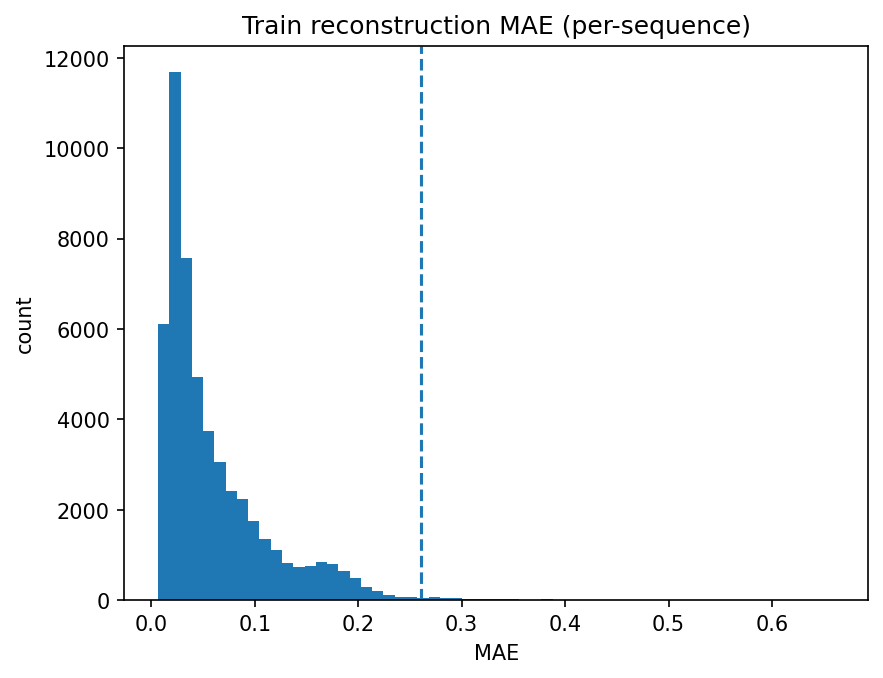
\includegraphics[width=\textwidth]{task14_train_mae_hist.png}
\caption{task 14 -- threshold 0,2609}
\end{subfigure}
\hfill
\begin{subfigure}{0.49\textwidth}
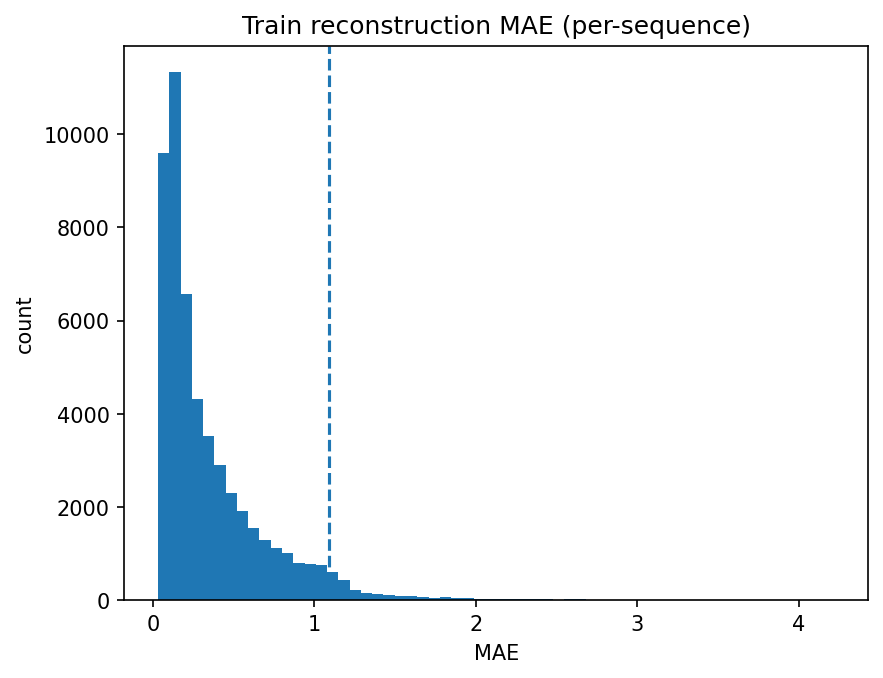
\includegraphics[width=\textwidth]{exp15b_train_mae_hist.png}
\caption{EXP15b -- threshold 1,0892}
\end{subfigure}
\caption{Distribuição do MAE de treino (canal-alvo) e o threshold
\texttt{robust\_mad} resultante, para cada candidato. A cauda longa à
direita é exatamente o padrão que motiva usar mediana+MAD em vez de
média+desvio-padrão -- poucos pontos de MAE alto no treino já inflam
\texttt{mean\_std} a um patamar que a série inteira nunca cruza.}
\label{fig:trainmaehist}
\end{figure}

\subsection{Camada de pós-processamento}

Antes de virar um ponto anômalo reportado, a detecção passa por quatro
filtros -- todos os quatro atuam sobre a saída do modelo já treinado,
sem alterar pesos nem o threshold em si (Figura~\ref{fig:pipeline}):

\begin{enumerate}[leftmargin=1.4em]
  \item \textbf{Máscara operacional} (Seção~\ref{sec:mascara-migracao}) --
    suprime detecção fora do estado \texttt{on}.
  \item \textbf{Portão de rampa} (\texttt{LOAD\_GATE\_SENSOR=T5\_AVG\_A},
    \texttt{RAMP\_MAX=50°C/h}) -- suprime durante manobra de carga
    legítima.
  \item \textbf{Portão de volatilidade}
    (\texttt{VOLATILITY\_GATE\_THRESHOLD=0,1745}, janela de 30\,min) --
    suprime durante vibração elevada persistente e fisicamente
    plausível.
  \item \textbf{Bloqueio gradual} (\texttt{GATE\_ESCAPE\_MULTIPLIER=1,5},
    Seção~\ref{sec:migracao}) -- um ponto cujo MAE bruto ultrapassa
    $\text{threshold} \times 1{,}5$ escapa do bloqueio de qualquer
    portão, mesmo sem saber qual bloqueou nem por quê. Nasceu do
    episódio 2026-01-29 do EXP13 (dois portões bloqueando
    simultaneamente uma detecção real) e é reaproveitado sem alteração
    no EXP15b.
\end{enumerate}

\begin{figure}[H]
\centering
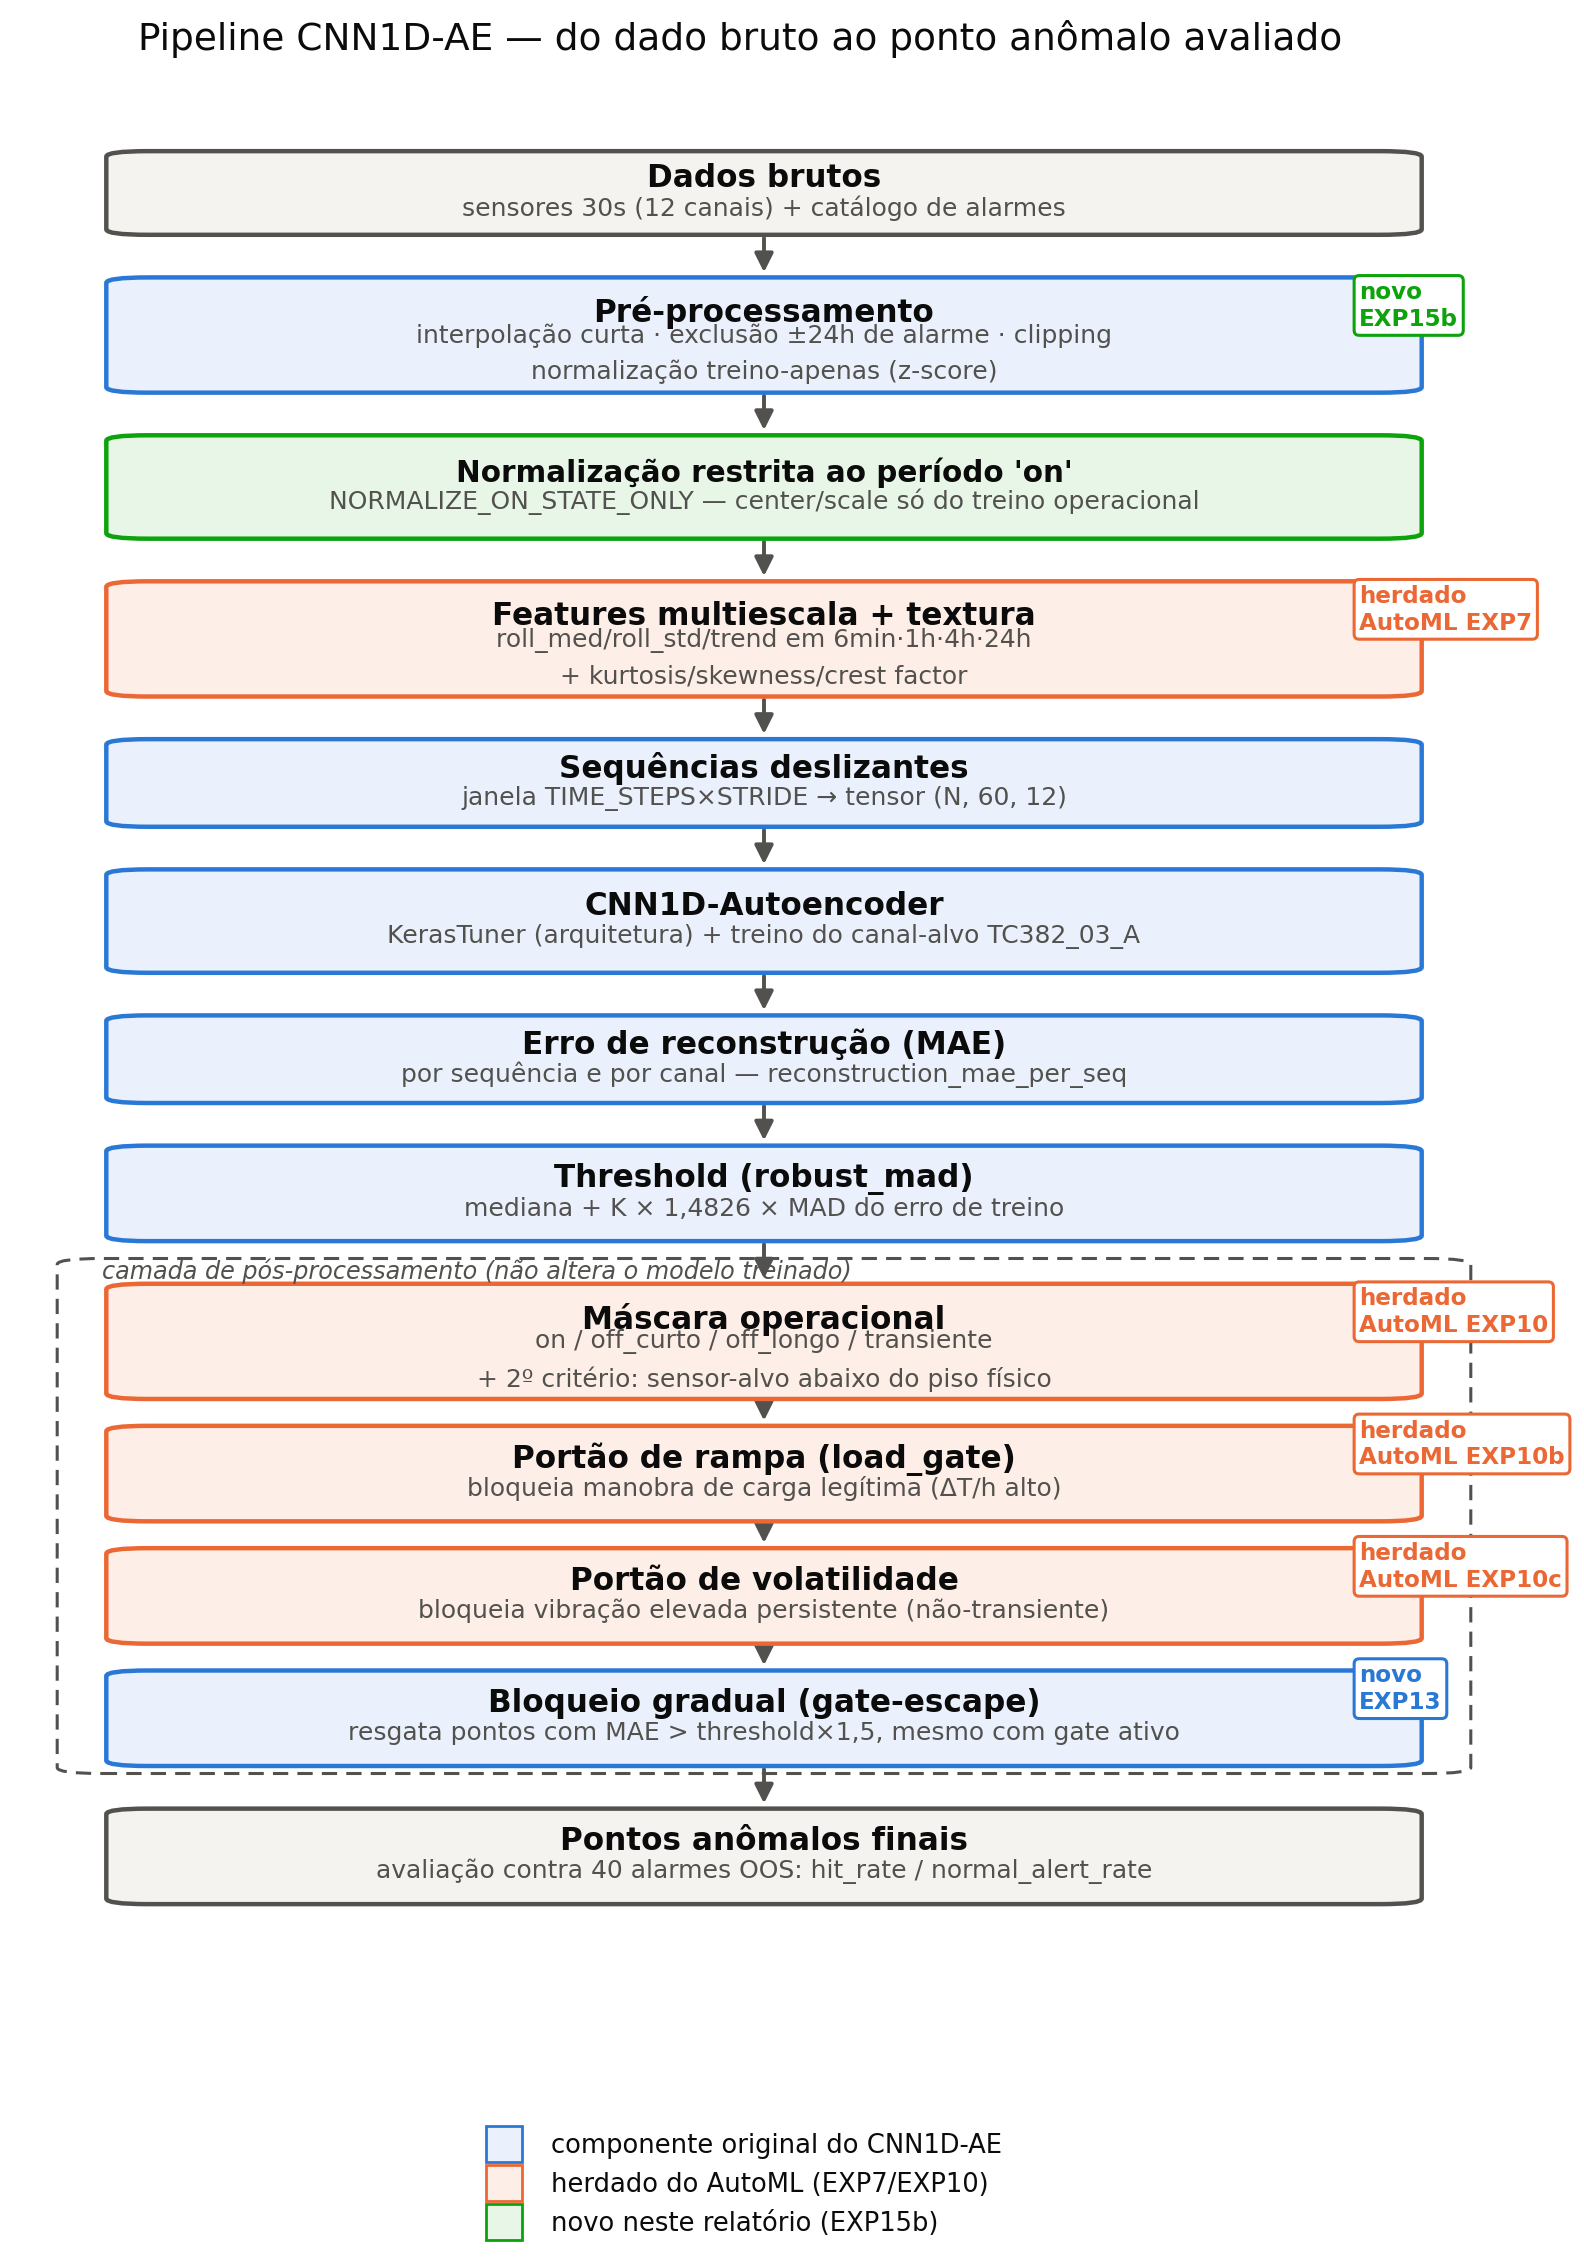
\includegraphics[width=0.82\textwidth]{fig_pipeline_esquema.png}
\caption{Esquema completo da pipeline, do dado bruto ao ponto anômalo
avaliado. Azul: componentes originais do CNN1D-AE. Laranja: mecanismos
herdados do AutoML (Seção~\ref{sec:migracao}). Verde: contribuição nova
deste relatório.}
\label{fig:pipeline}
\end{figure}

\subsection{Contribuição nova: normalização restrita ao período operacional}
\label{sec:normalizacao-on-state}

A investigação que motiva este relatório partiu de dois episódios reais
não detectados pelo candidato de referência anterior (task~14,
Seção~\ref{sec:resultados}). O episódio de \textbf{2026-04-14} revelou
uma falha estrutural na normalização: \texttt{normalize\_train\_only}
(\texttt{preprocess.py}) sempre calculou \texttt{center}/\texttt{scale}
sobre \emph{todo} o \texttt{df\_normal\_fit} (dados de treino, excluindo
só janelas de alarme e gaps longos) -- \textbf{sem} excluir os períodos
de parada/partida da turbina. Como $\sim$42\% do treino tem
\texttt{TC382\_03\_A}$<$100°C (turbina desligada), o desvio-padrão
usado para o z-score é inflado por essa mistura bimodal: 51,1°C
considerando só o período operando versus 323,0°C misturado com
parada/partida -- quase 6,3$\times$ maior.

O efeito prático: um desvio real de +115°C \emph{dentro} da operação
normal (o episódio de 2026-04-14) produz um z-score de apenas 1,22 com
as estatísticas contaminadas, contra 2,22 se calculado só sobre o
período operacional -- quase metade da magnitude estatística
disponível para o autoencoder aprender a distinguir esse desvio do
ruído normal.

\textbf{Implementação} (\texttt{NORMALIZE\_ON\_STATE\_ONLY},
\texttt{config.py} + \texttt{preprocess.py} + \texttt{pipeline.py}):
\texttt{normalize\_train\_only} recebe um \texttt{stats\_mask} opcional
-- quando fornecido, \texttt{center}/\texttt{scale} são calculados só
sobre as linhas de \texttt{df\_normal\_fit} onde
\texttt{operational\_state=='on'}. Duas decisões de design deliberadas:

\begin{itemize}[leftmargin=1.4em]
  \item \textbf{Não filtra as linhas de treino em si} -- as sequências
    de treino continuam contíguas no tempo (sem remover janelas
    off/partida e recolar os pedaços), evitando descontinuidades
    artificiais nas sequências que o autoencoder aprende a reconstruir.
    Só as \emph{estatísticas} usadas para normalizar mudam.
  \item \textbf{Cálculo do estado operacional antecipado} -- no
    \texttt{run\_one\_group}, o cálculo de \texttt{state}
    (\seqsplit{build\_operational\_state}) foi movido para antes de
    \texttt{normalize\_train\_only} (antes rodava só depois, para
    mascarar detecções). Comportamento idêntico ao anterior quando a
    flag está desligada (\texttt{False} por default) -- nenhum
    experimento existente muda de resultado.
\end{itemize}

Esse ganho de sinal tem um efeito colateral que a Seção~\ref{sec:discussao}
discute: os períodos off/partida continuam nas sequências de treino,
agora normalizados com um desvio-padrão menor -- um valor de $\sim$33°C
(desligado) vira um z-score de $\approx{-}12{,}7$ em vez de
$\approx{-}1{,}1$, forçando o autoencoder a reconstruir transições
artificialmente amplificadas. Isso exigiu uma recalibração de threshold
não-trivial (não um simples reescalonamento linear) para chegar ao
candidato final.

% =====================================================================
\section{Resultados}
\label{sec:resultados}
% =====================================================================

\subsection{Evolução do candidato}

A Tabela~\ref{tab:evolucao} e a Figura~\ref{fig:comparativo} mostram a
evolução completa, do melhor candidato AutoML (referência externa) até
o EXP15b, todos avaliados na mesma régua (40 alarmes OOS de
\texttt{TC382\_03\_A}/\texttt{T5\_AVG\_A}).

\begin{table}[H]
\centering
\begin{tabular}{@{}lccl@{}}
\toprule
\textbf{Candidato} & \textbf{hit\_rate} & \textbf{FP} & \textbf{Observação} \\
\midrule
AutoML EXP10c (referência) & 92,5\% (37/40) & 0,35\% & \texttt{ocsvm}, 3 portões, ver Seção~\ref{sec:migracao} \\
CNN1D-AE task 13 & 60,0\% (24/40) & 0,17\% & \texttt{THRESH\_STD\_K=7,0}, sem gate-escape \\
CNN1D-AE task 14 (anterior) & 75,0\% (30/40) & 0,22\% & + gate-escape (resgata 2026-01-29) \\
\textbf{CNN1D-AE EXP15b (novo)} & \textbf{77,5\% (31/40)} & \textbf{0,30\%} & + normalização on-state + \texttt{K=4,5} \\
\bottomrule
\end{tabular}
\caption{Evolução do candidato de referência do CNN1D-AE, com o melhor
candidato AutoML como teto de referência.}
\label{tab:evolucao}
\end{table}

\begin{figure}[H]
\centering
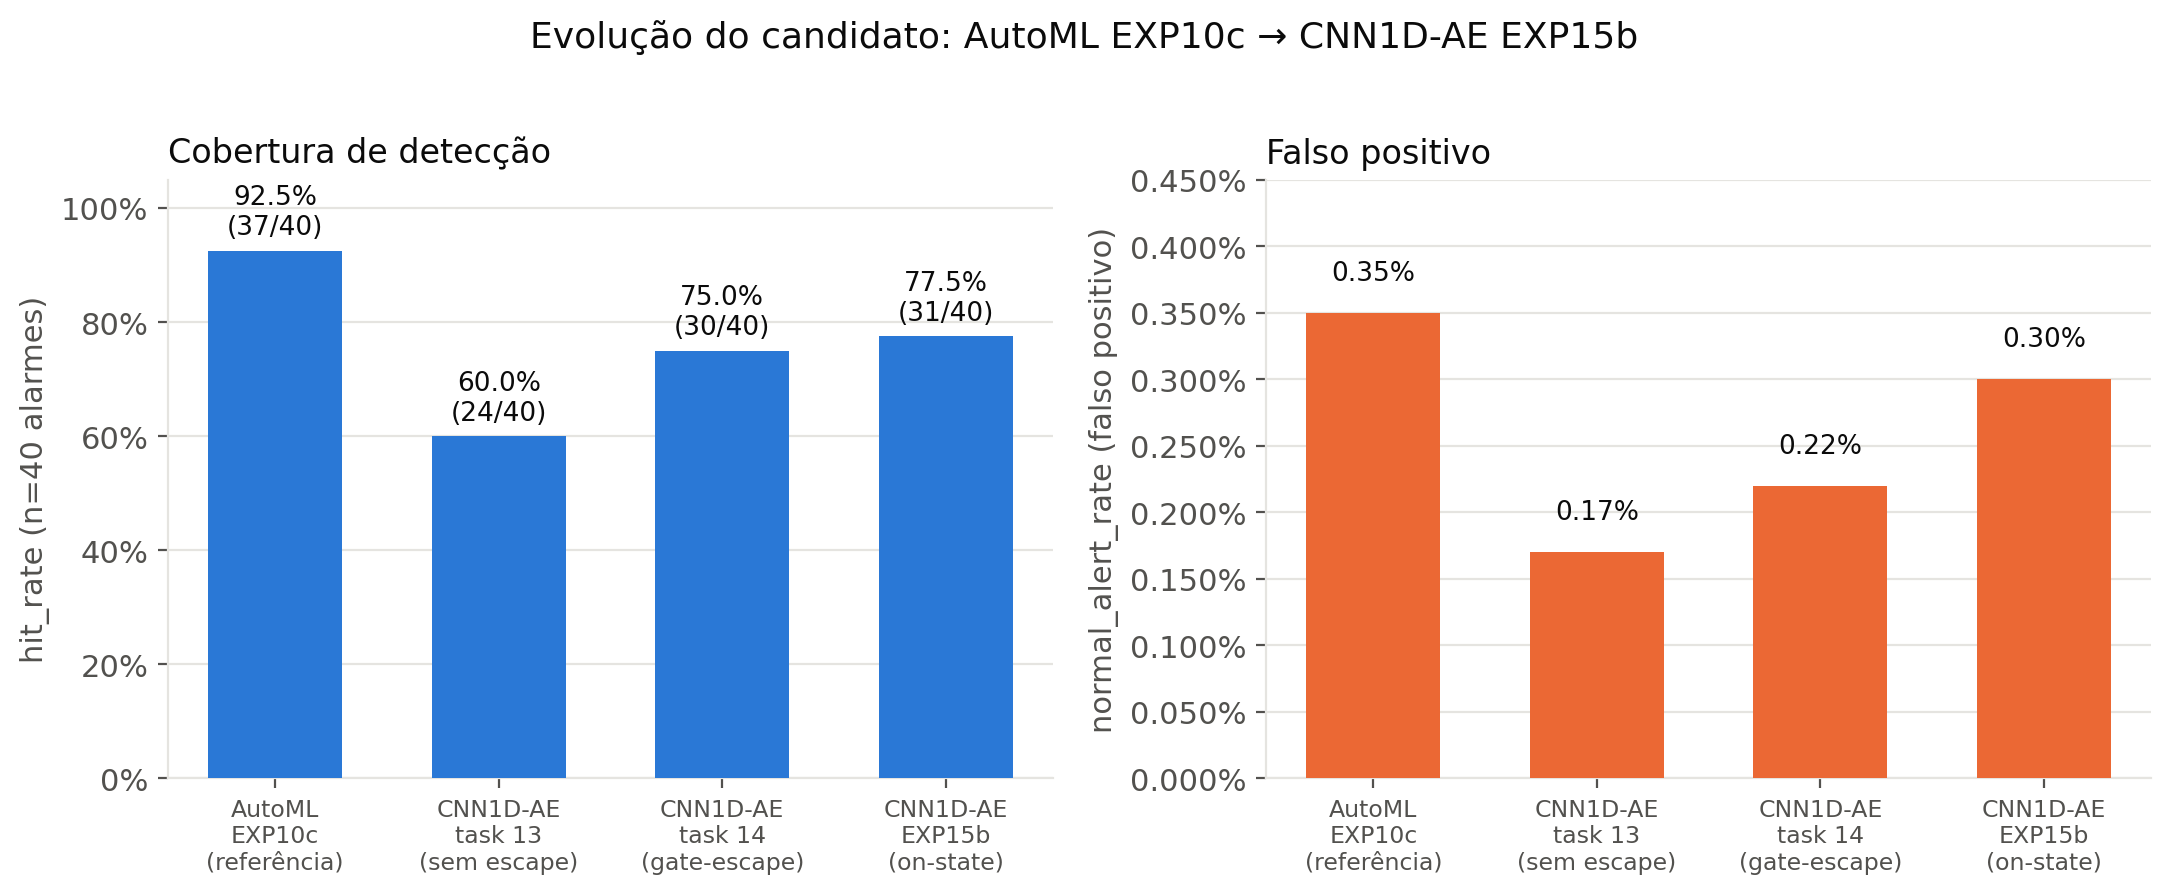
\includegraphics[width=\textwidth]{fig_comparativo_metricas.png}
\caption{\texttt{hit\_rate} e falso positivo (\texttt{normal\_alert\_rate})
ao longo da evolução do candidato. O EXP15b supera o candidato anterior
(task~14) nos dois eixos simultaneamente... exceto pelo FP, que sobe
$\sim$37\% relativo (0,22\%$\to$0,30\%) -- ainda assim bem abaixo do
teto do AutoML (0,35\%).}
\label{fig:comparativo}
\end{figure}

\subsection{Estudo de caso: o episódio de 2026-04-14}

A Figura~\ref{fig:caso0414} mostra o mecanismo do resgate diretamente
nos dados. No painel superior, a temperatura bruta de
\texttt{TC382\_03\_A} sobe suavemente de $\sim$677°C (13/04, 12h) para
$\sim$793°C (14/04, 12h) ao longo de $\sim$24h -- sem descontinuidade
local que uma janela de 30\,min pudesse capturar como ``forma''
anômala. No painel inferior, o erro de reconstrução do canal-alvo: a
curva do candidato anterior (task~14, azul) mal reage --  fica sempre
abaixo do seu próprio threshold (0,26) mesmo com a temperatura 115°C
acima do início da janela. A curva do EXP15b (laranja) cruza claramente
o seu threshold (1,09) já na madrugada de 14/04 e se mantém acima na
maior parte da janela, incluindo nos três horários de alarme reais
(HI às 00h12, HI às 10h07, HIHI às 12h01, marcados em vermelho).

\begin{figure}[H]
\centering
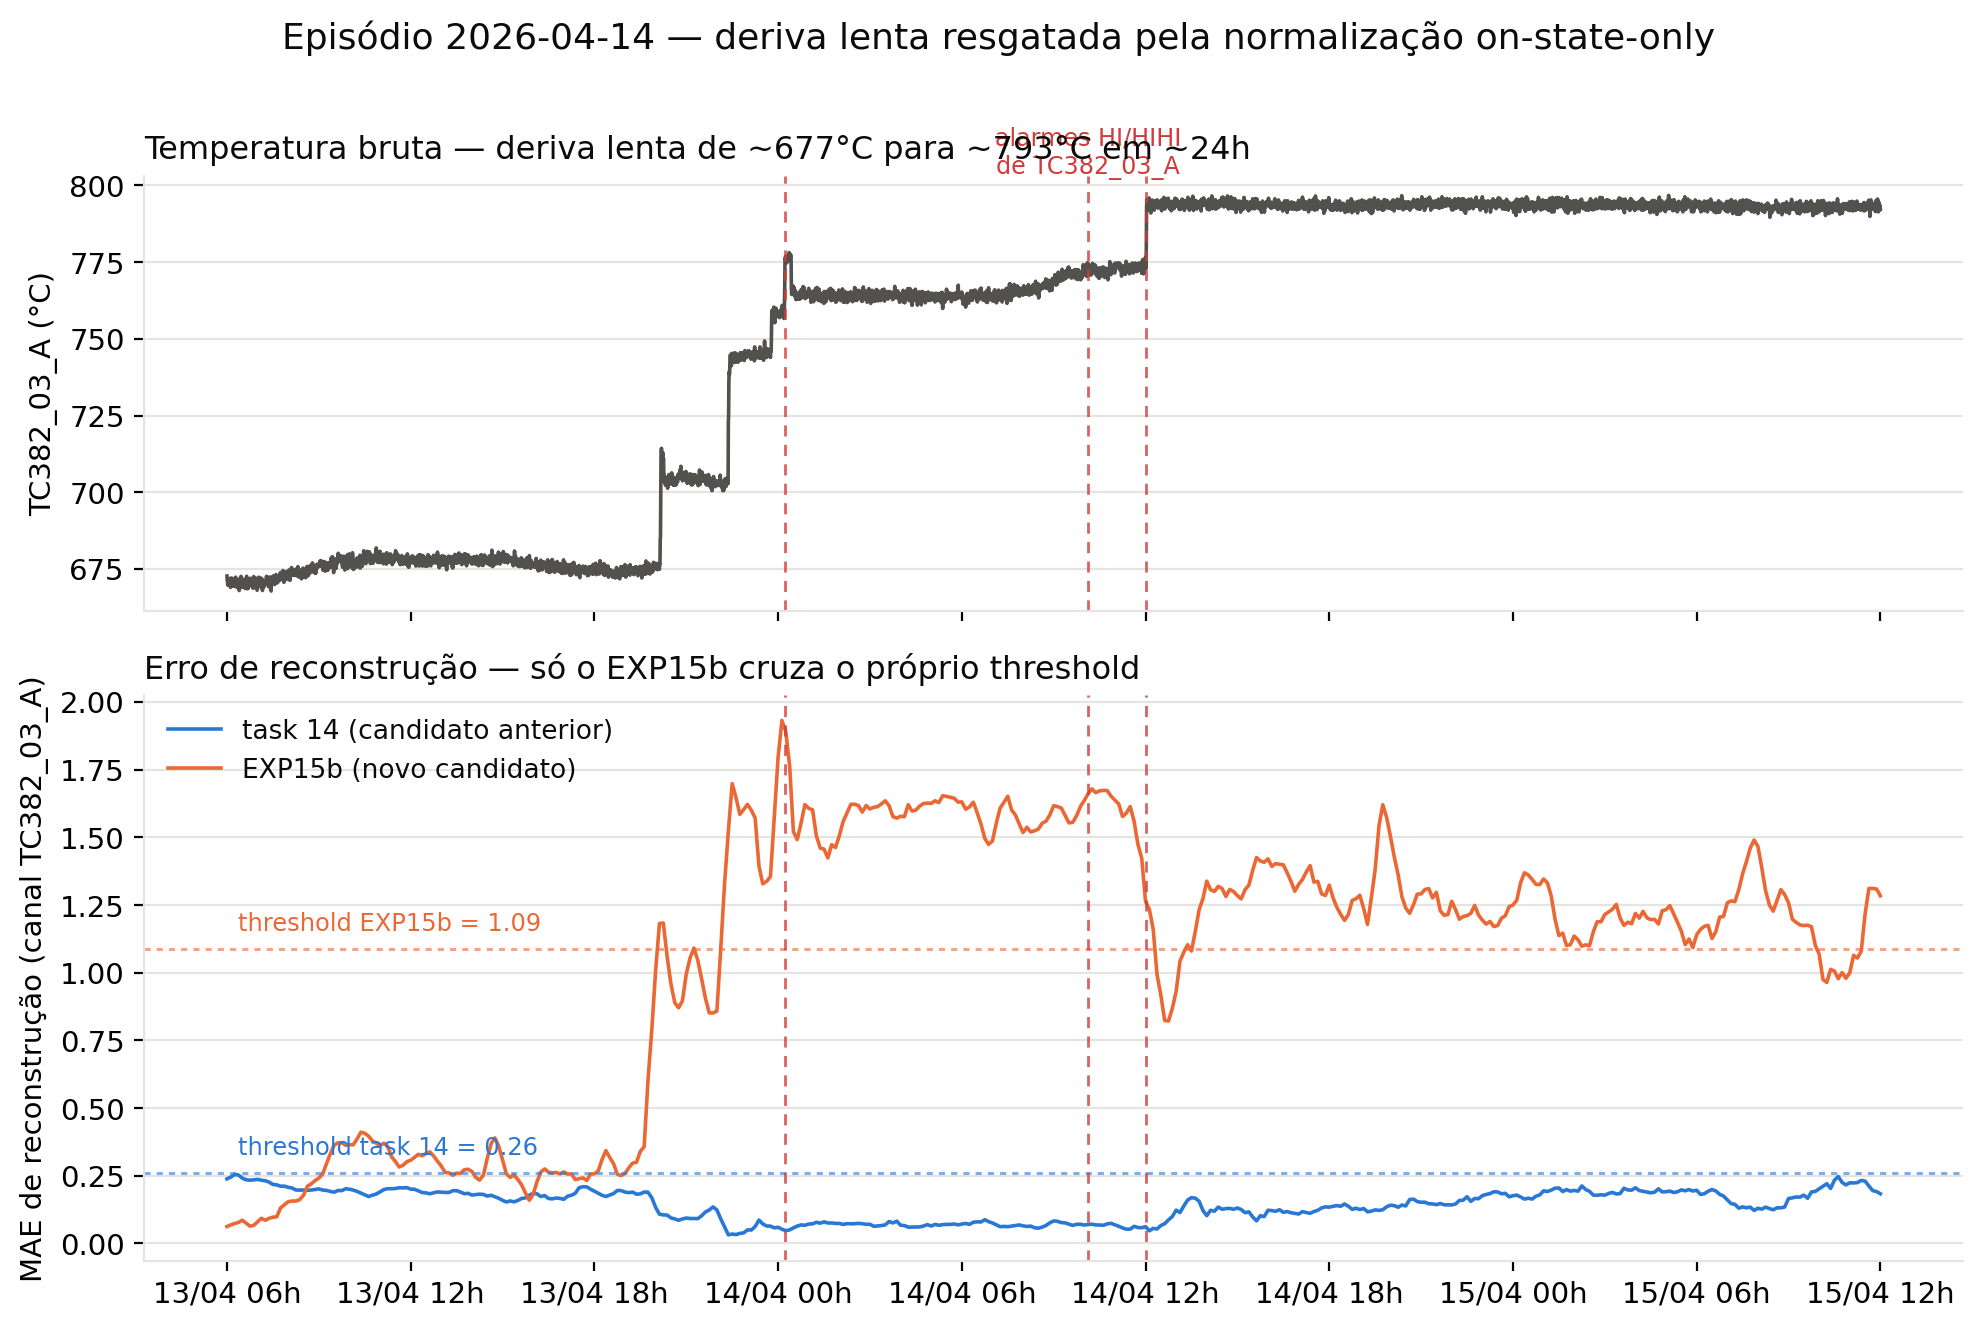
\includegraphics[width=0.92\textwidth]{fig_caso_0414.png}
\caption{Episódio 2026-04-14: temperatura bruta (topo) e erro de
reconstrução dos dois candidatos (base), com os respectivos thresholds.
Note que os dois eixos de MAE não são diretamente comparáveis em escala
absoluta -- a normalização de entrada mudou entre os dois candidatos --
o que importa é a posição de cada curva \emph{relativa ao seu próprio}
threshold.}
\label{fig:caso0414}
\end{figure}

Confirmação no nível de ponto (após máscara operacional e portões):
138 e 161 pontos anômalos nas janelas de $\pm$24h dos dois principais
alarmes do dia, mesmo com \texttt{load\_gate}/\texttt{volatility\_gate}
ativos na região -- resgatados pelo \emph{gate-escape}, o mesmo
mecanismo que já havia resgatado o episódio 2026-01-29 no candidato
anterior.

\subsection{Classificação dos alarmes por qualidade de detecção}

Além da métrica agregada \texttt{hit\_rate} (que só pergunta ``existe
algum ponto anômalo na janela de $\pm$24h?''), classificamos cada um
dos 40 alarmes pelo tempo de antecedência da primeira detecção dentro
dessa janela: \textbf{preditivo} (primeira detecção antes do alarme, até
20h de antecedência), \textbf{suspeito} (antecedência $>$20h --
padrão já documentado de artefato: quando a detecção está perto do teto
da janela de avaliação, é mais provável ser coincidência da janela ser
larga do que sinal precursor real), \textbf{reativo} (detecção no
instante do alarme ou depois) e \textbf{sem detecção}.

\begin{figure}[H]
\centering
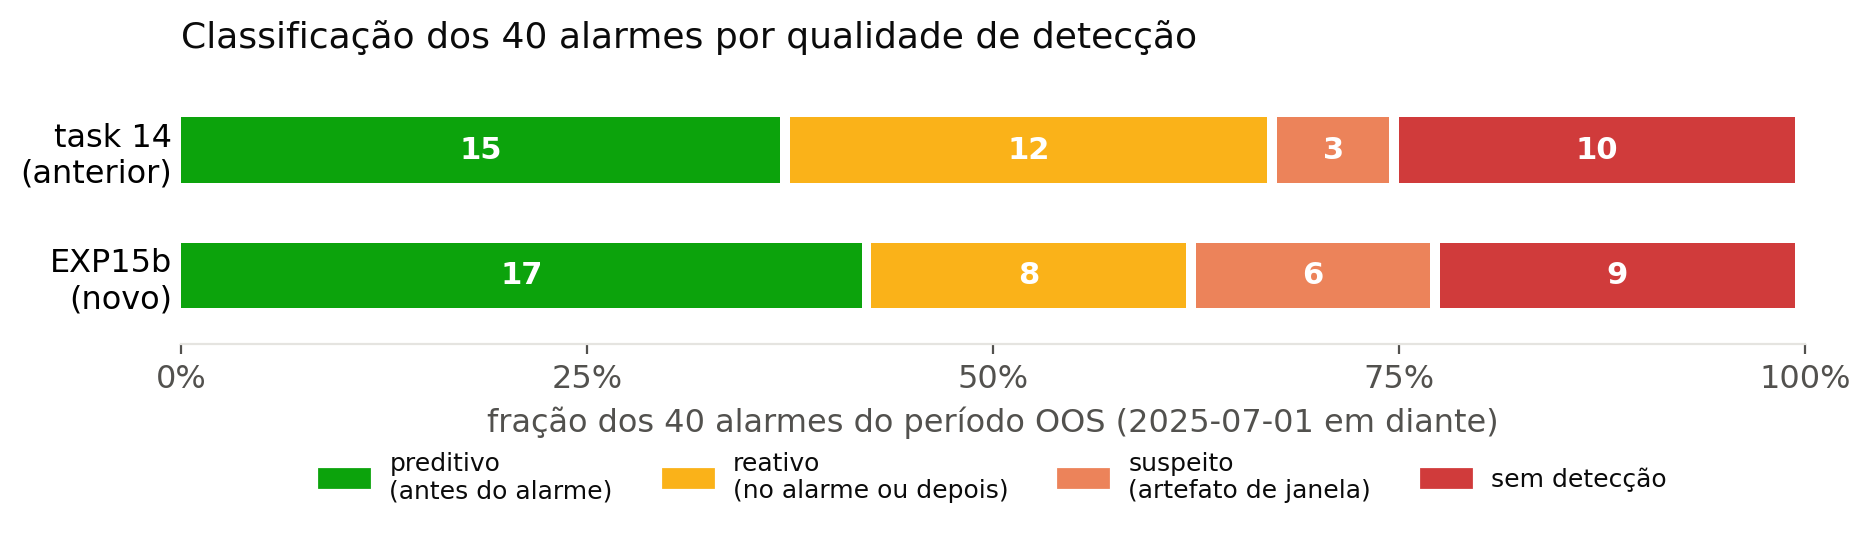
\includegraphics[width=0.92\textwidth]{fig_categorias_deteccao.png}
\caption{Classificação automática dos 40 alarmes do período OOS por
qualidade de detecção (metodologia de antecedência descrita no texto).
Dos 40 alarmes, 4 são falhas confirmadas de comunicação/instrumento
(\texttt{Comm Fail}/\texttt{Out of Serv} no dado bruto do SCADA), sem
precursor físico esperado -- não removidos desta contagem para manter a
comparação simples, mas documentados em detalhe em
\texttt{docs/analise\_cnn1dae\_exp13.md}.}
\label{fig:categorias}
\end{figure}

O EXP15b desloca massa de ``reativo'' para ``preditivo''
(15$\to$17, e sobretudo reativo caindo de 12 para 8) e reduz ``sem
detecção'' de 10 para 9 -- ganho líquido pequeno em contagem bruta, mas
o episódio 2026-04-14 (3 alarmes do mesmo dia, antes inteiramente
perdido) agora conta como detecção real, e o aumento de ``suspeito''
(3$\to$6) é o preço de um modelo genuinamente mais sensível: mais casos
próximos do teto de 24h da janela de avaliação, consistente com um
threshold mais permissivo em valor absoluto de sinal (mesmo mantendo o
mesmo critério relativo).

\subsubsection{Antecedência de detecção, caso a caso}

A Figura~\ref{fig:leadtime} detalha a métrica por trás da classificação
da Figura~\ref{fig:categorias}: para cada um dos 40 alarmes, quantas
horas antes (ou depois) do timestamp oficial do alarme a primeira
detecção ocorreu, para os dois candidatos lado a lado. Além de permitir
auditar caso a caso -- por exemplo, confirmar visualmente que os três
alarmes de 2026-04-14 têm marcador (triângulo laranja) só para o
EXP15b, e nenhum marcador (círculo azul) para a task~14 -- o gráfico
deixa claro um padrão que a métrica agregada esconde: quando os dois
candidatos detectam o \emph{mesmo} alarme, a antecedência é quase
sempre muito parecida entre eles (os pares de marcadores tendem a cair
próximos um do outro no eixo x) -- a recalibração não mudou
\emph{quando} um alarme já detectado seria pego, só ampliou o
\emph{conjunto} de alarmes detectados.

\begin{figure}[H]
\centering
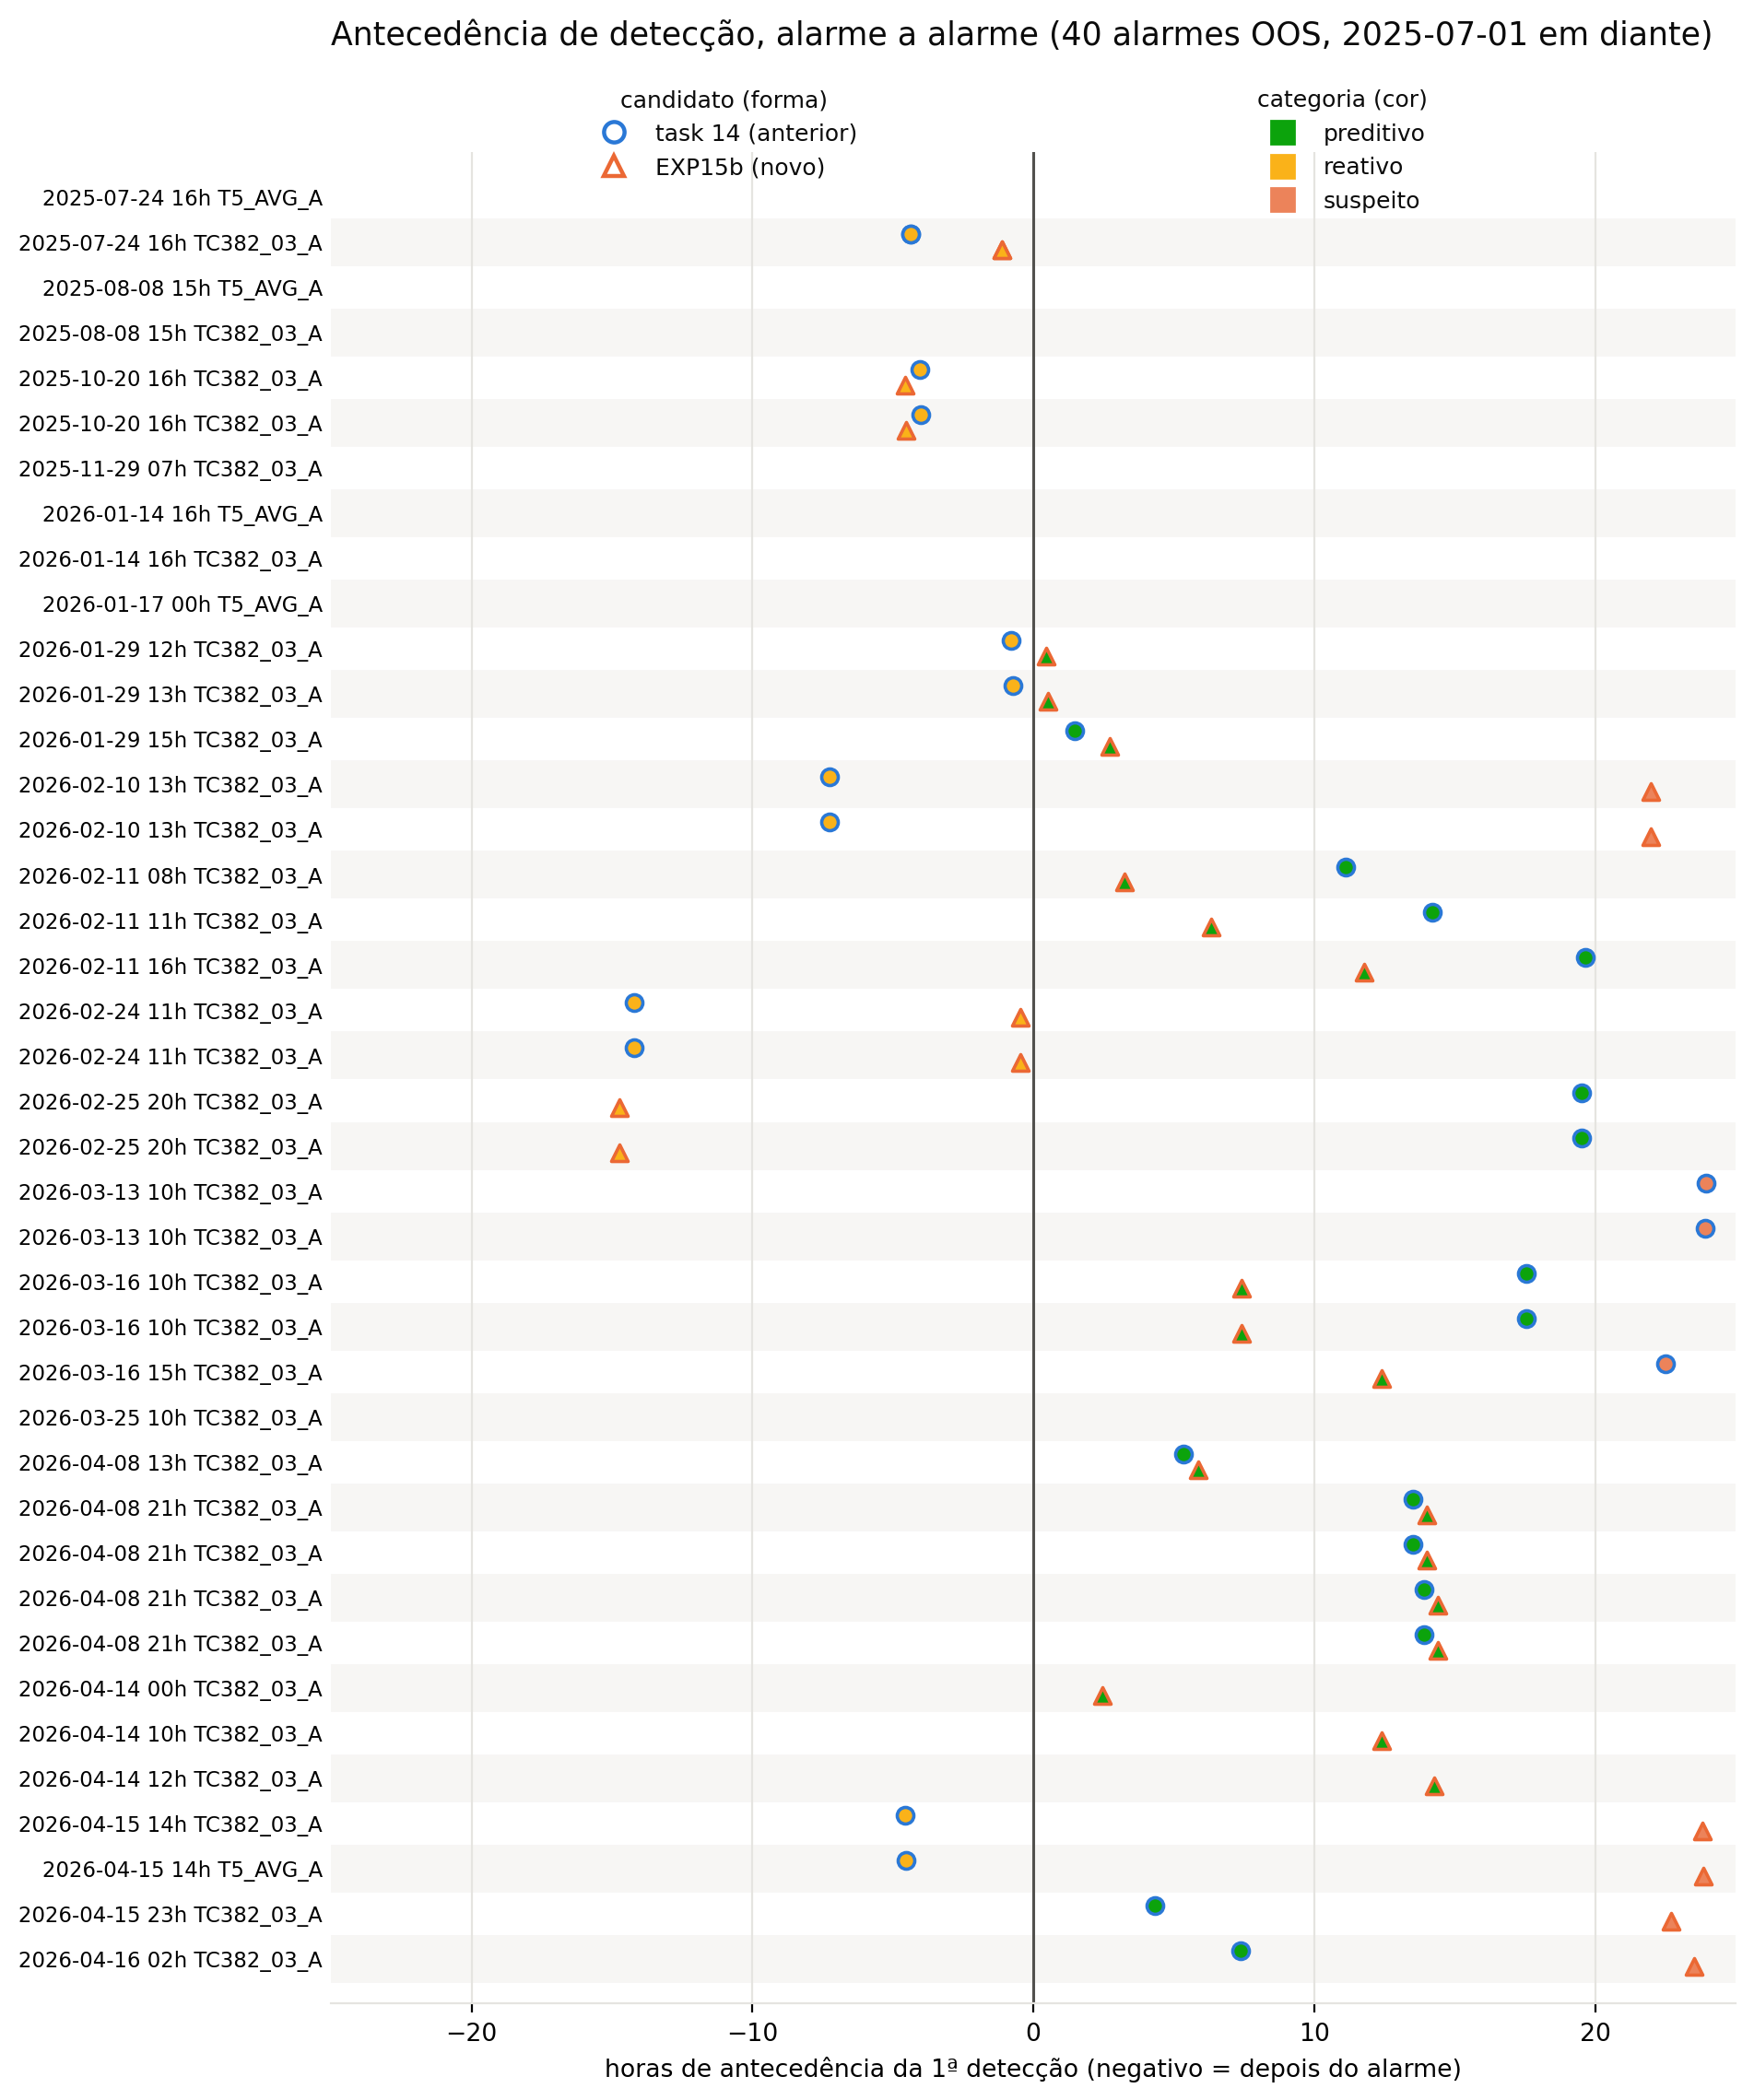
\includegraphics[width=0.94\textwidth]{fig_lead_time_por_alarme.png}
\caption{Antecedência da primeira detecção, alarme a alarme (40 alarmes
OOS, ordem cronológica). Círculo azul = task~14; triângulo laranja =
EXP15b; cor de preenchimento = categoria (Figura~\ref{fig:categorias}).
Linha vertical em 0 = instante do alarme. Ausência de marcador = alarme
sem detecção naquele candidato.}
\label{fig:leadtime}
\end{figure}

A Figura~\ref{fig:leadtimedist} resume só as detecções preditivas (as
que efetivamente anteciparam o alarme) numa distribuição comparável. O
EXP15b tem mais detecções preditivas (17 vs. 15), mas com antecedência
\emph{menor} em média (8,5h vs. 12,8h; mediana 7,4h vs. 13,9h) -- os
casos novos que o EXP15b passou a capturar (incluindo os três de
2026-04-14, com antecedência de 4,3h a 7,4h) tendem a ser detecções
mais próximas do instante do alarme que a média dos casos que o
candidato anterior já capturava, puxando a distribuição toda para
antecedências menores.

\begin{figure}[H]
\centering
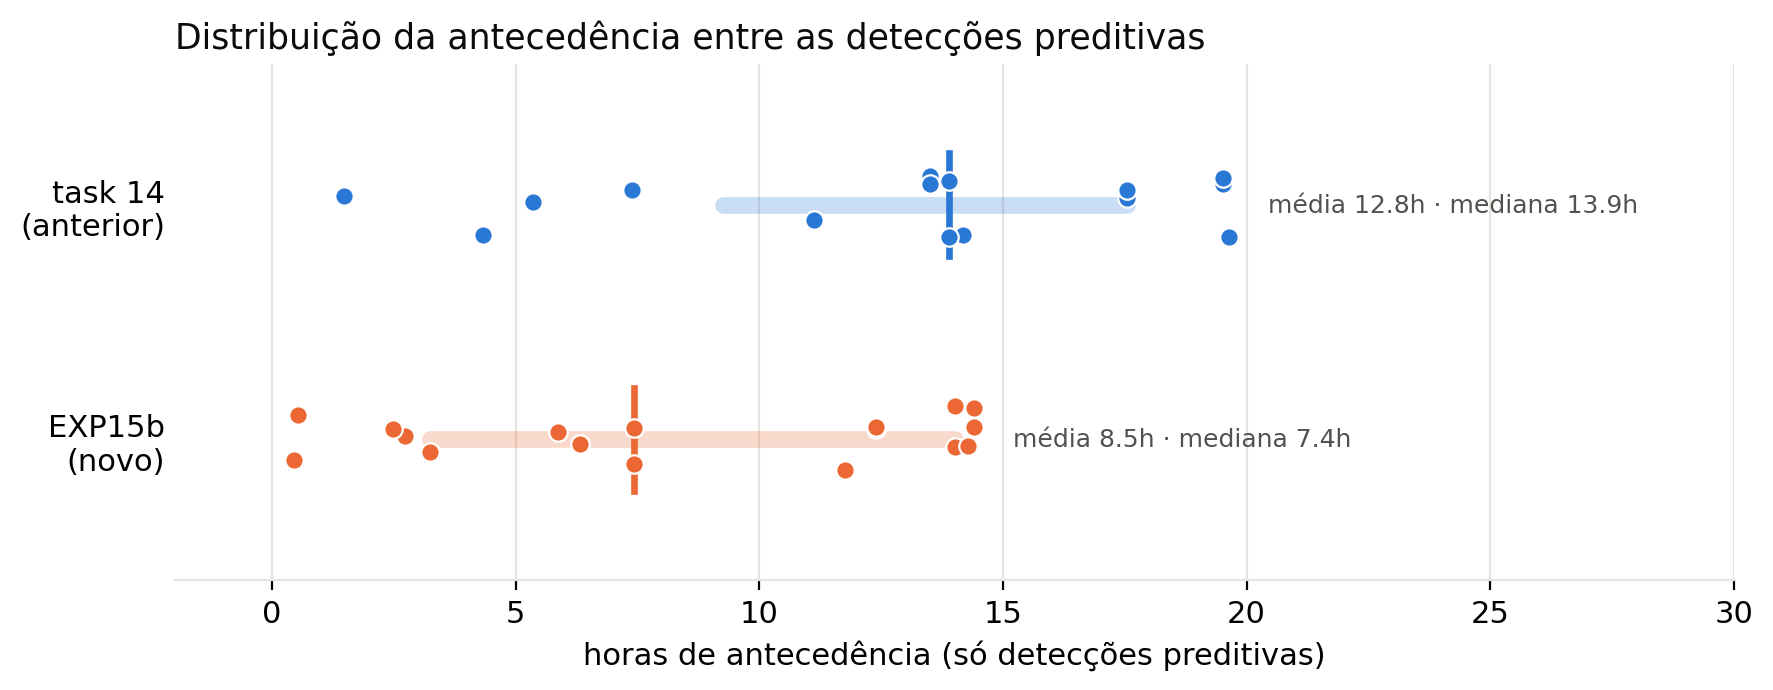
\includegraphics[width=0.92\textwidth]{fig_lead_time_distribuicao.png}
\caption{Distribuição da antecedência (horas) entre as detecções
classificadas como preditivas, por candidato. Barra horizontal = IQR;
traço vertical = mediana.}
\label{fig:leadtimedist}
\end{figure}

\subsection{Variação entre sementes de retreino (seed-sweep)}
\label{sec:seedsweep}

A comparação seed-sweep contra seed-sweep
(Figura~\ref{fig:seedsweep}) mostra que o EXP15b supera o candidato
anterior em \textbf{todos} os pontos -- semente principal, média,
mínimo e máximo do sweep:

\begin{table}[H]
\centering
\begin{tabular}{@{}lccccc@{}}
\toprule
\textbf{Candidato} & \textbf{seed principal} & \textbf{média sweep} & \textbf{std} & \textbf{mín} & \textbf{máx} \\
\midrule
task 14 (anterior) & 75,0\% & 50,0\% & $\pm$7,7pp & 37,5\% & 57,5\% \\
EXP15b (novo) & 77,5\% & 60,6\% & $\pm$9,9pp & 47,5\% & 75,0\% \\
\bottomrule
\end{tabular}
\caption{Seed-sweep (\texttt{SEED\_SWEEP\_N=4}, sementes 43--46) de
cada candidato. O desvio-padrão em pontos percentuais é maior no
EXP15b, mas o coeficiente de variação (std/média) é praticamente igual
entre os dois (16,3\% vs. 15,4\%) -- o EXP15b não é ``mais instável'',
só parte de uma base mais alta.}
\label{tab:seedsweep}
\end{table}

\begin{figure}[H]
\centering
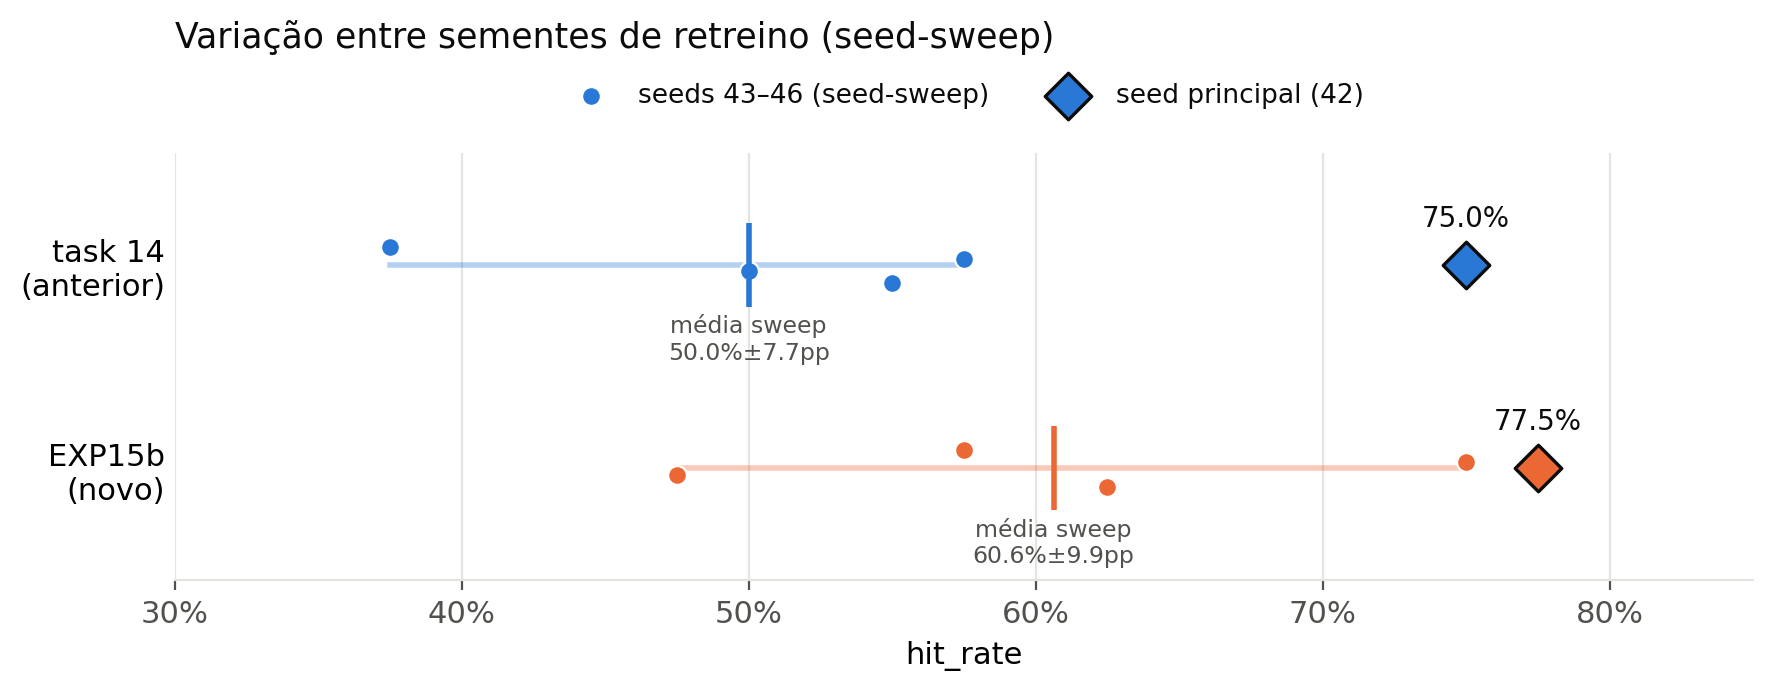
\includegraphics[width=0.92\textwidth]{fig_seed_sweep.png}
\caption{Dispersão do \texttt{hit\_rate} entre a semente principal (42,
losango) e as 4 sementes do sweep (círculos, com a média marcada por um
traço vertical), para os dois candidatos.}
\label{fig:seedsweep}
\end{figure}

\subsection{Séries completas com anomalias marcadas}

As Figuras~\ref{fig:series-task14} e~\ref{fig:series-exp15b} mostram a
série bruta completa de \texttt{TC382\_03\_A} de cada candidato, com o
estado operacional (faixa inferior: verde=ligada, laranja=desligada)
gerada automaticamente pela pipeline -- referência visual da amplitude
completa da série (incluindo os $\sim$1,9 anos de dados de treino) e do
padrão intermitente de liga/desliga que motiva a máscara operacional
(Seção~\ref{sec:mascara-migracao}).

\begin{figure}[H]
\centering
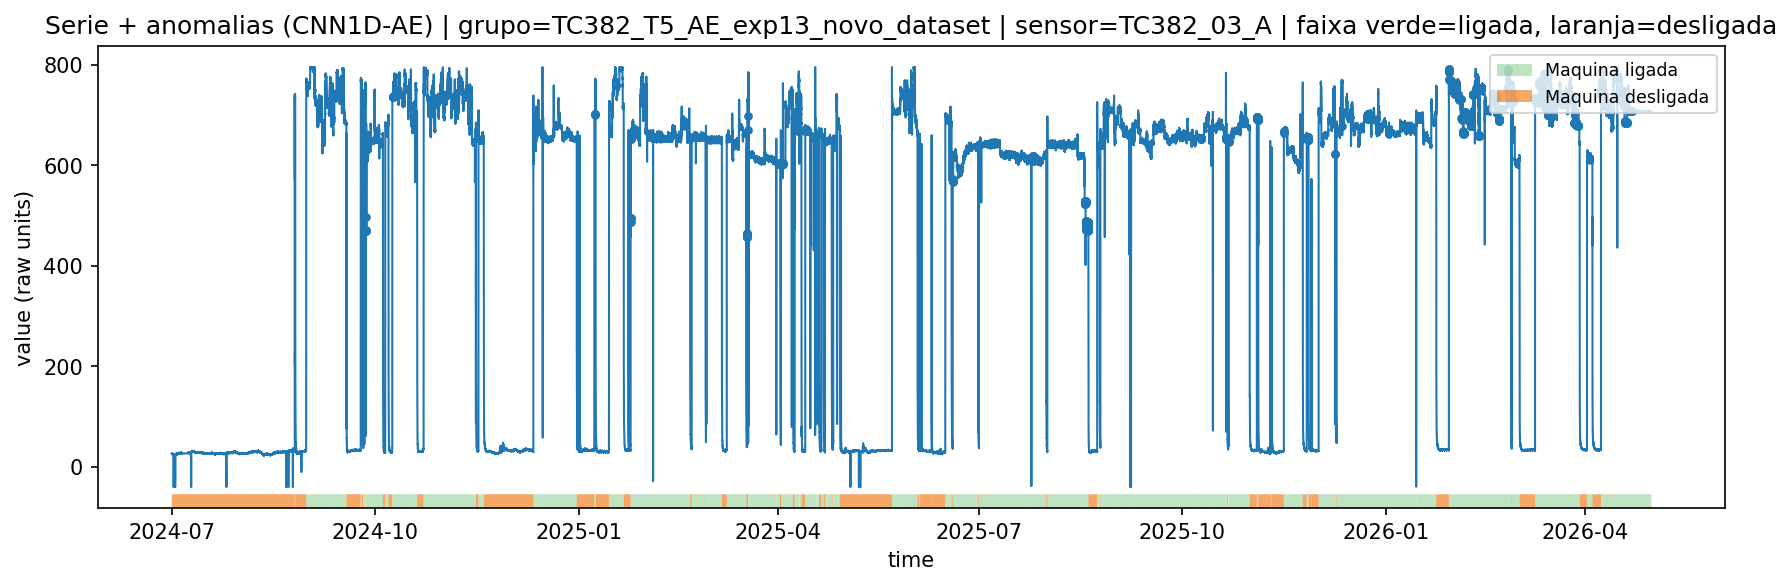
\includegraphics[width=0.92\textwidth]{task14_series_with_anomalies_TC382_03_A.png}
\caption{Série completa de \texttt{TC382\_03\_A} -- candidato anterior
(task 14).}
\label{fig:series-task14}
\end{figure}

\begin{figure}[H]
\centering
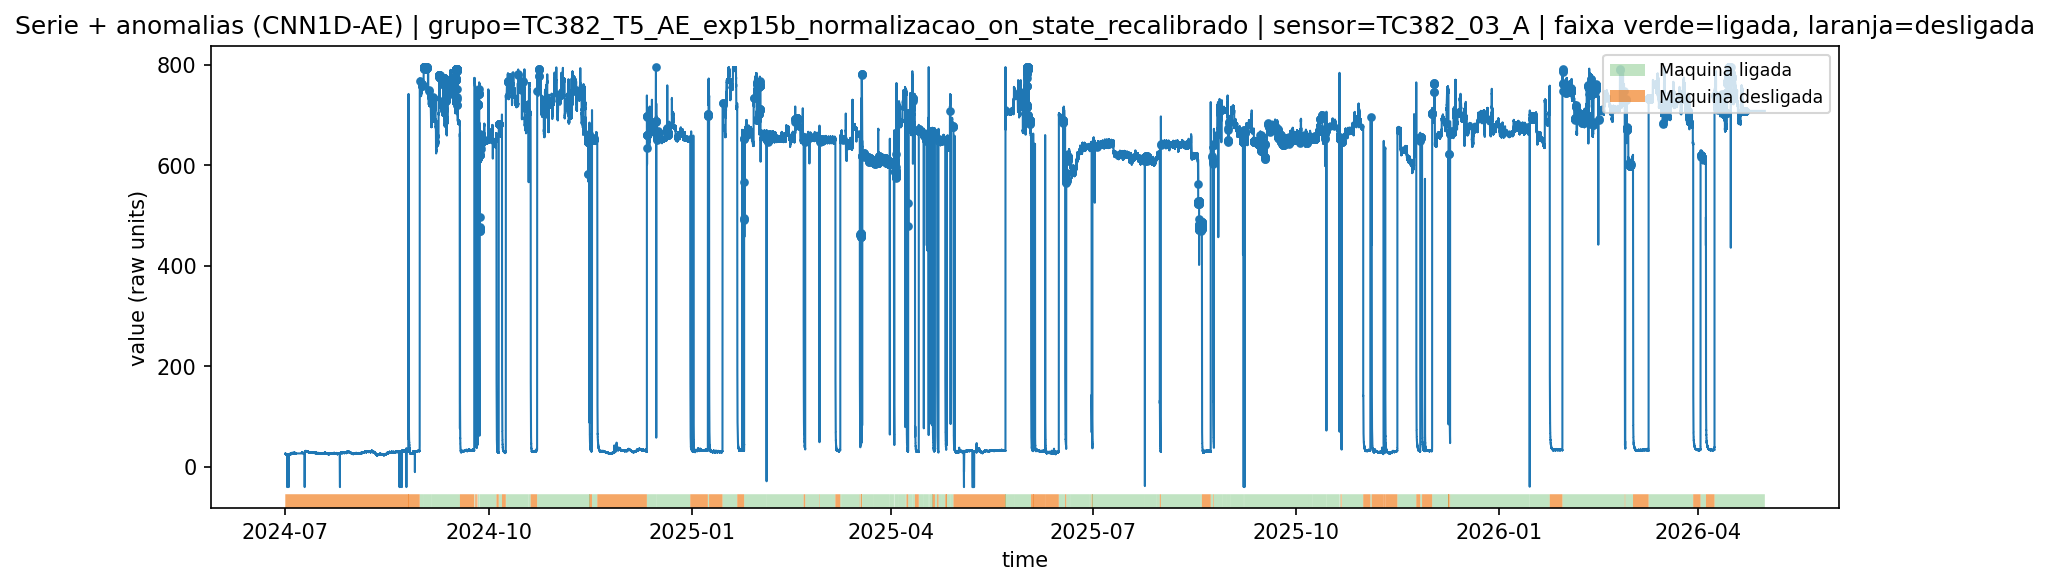
\includegraphics[width=0.92\textwidth]{exp15b_series_with_anomalies_TC382_03_A.png}
\caption{Série completa de \texttt{TC382\_03\_A} -- candidato novo
(EXP15b).}
\label{fig:series-exp15b}
\end{figure}

% =====================================================================
\section{Discussão}
\label{sec:discussao}
% =====================================================================

\subsection{Tentativa de mitigação de variância rejeitada}

Antes de aceitar o EXP15b como candidato final, testamos se
\texttt{THRESH\_MODE=target\_rate} (fixar a \emph{taxa} de anomalia do
treino em vez de mediana+MAD) reduziria a variância de semente sem
custo. O resultado foi negativo: o threshold saiu 2,3$\times$ mais alto
(2,4743 vs. 1,0892), porque o quantil top-0,3\% da distribuição de erro
de treino é bem mais extremo que mediana+$K\times$MAD nesta
distribuição específica. \texttt{hit\_rate} da semente principal caiu
para 15,0\% (6/40); a variância de fato caiu (std $\pm$3,2pp vs.
$\pm$9,9pp), mas porque as 4 sementes do sweep convergiram para um piso
de detecção quase inútil (5,0\%--12,5\%), não porque a calibração
melhorou -- e o pico de MAE do episódio 2026-04-14 (1,93) ficou abaixo
desse threshold mais alto, ou seja, essa variante voltava a perder o
episódio que motivou todo o EXP15/EXP15b. \texttt{target\_rate} fica
descartado como modo de threshold para este pipeline nesta taxa-alvo.

\subsection{Limitações}

\begin{itemize}[leftmargin=1.4em]
  \item \textbf{Efeito colateral da normalização on-state} --
    (Seção~\ref{sec:normalizacao-on-state}) os períodos off/partida
    continuam nas sequências de treino, agora como outliers extremos em
    z-score. Não investigado se isso degrada a qualidade de
    reconstrução do autoencoder de forma mensurável além do efeito já
    observado na escala do threshold.
  \item \textbf{Amostra pequena do seed-sweep} ($N=4$) -- os números de
    variância da Seção~\ref{sec:seedsweep} têm incerteza estatística
    considerável; \texttt{SEED\_SWEEP\_N} maior daria uma leitura mais
    confiável antes de qualquer decisão que dependa fortemente do
    desvio-padrão exato.
  \item \textbf{Classificação preditivo/reativo/suspeito automatizada} --
    a Figura~\ref{fig:categorias} usa um critério de antecedência
    simples (limiar de 20h), mais simplificado que a auditoria manual
    caso a caso feita para o candidato anterior no
    \texttt{docs/analise\_cnn1dae\_exp13.md} (que cruzou cada caso com
    o dado bruto e o código de status do SCADA). As duas metodologias
    concordam no número de casos preditivos do candidato anterior (15),
    mas não foram desenhadas para produzir números idênticos em outras
    categorias.
  \item \textbf{Gap de cobertura para o AutoML} -- mesmo após o EXP15b,
    o CNN1D-AE (77,5\%) ainda fica 15\,pp atrás do melhor candidato
    AutoML (92,5\%). O EXP15b fecha parte do gap fechado por task~14
    (13,3\,pp$\to$4,2\,pp de cobertura genuína, conforme
    \texttt{analise\_cnn1dae\_exp13.md}) mas não o elimina.
\end{itemize}

\subsection{Pendências}

\begin{itemize}[leftmargin=1.4em]
  \item Decidir se o EXP15b substitui definitivamente a task~14 como
    candidato de produção, ou se o trade-off cobertura$\times$FP
    justifica manter os dois como opções calibráveis por operador.
  \item Investigar se filtrar diretamente as linhas de treino pelo
    estado operacional (em vez de só as estatísticas de normalização)
    resolve o efeito colateral de outliers extremos sem reintroduzir o
    problema original de descontinuidade de sequências -- por exemplo,
    treinando com sequências geradas separadamente por trecho contínuo
    de operação, sem concatenar através de um gap off/partida.
  \item O episódio de 2026-03-25 (bloqueio de gate por margem pequena,
    ver \texttt{analise\_cnn1dae\_exp13.md}) segue sem correção --
    candidato: um segundo \texttt{GATE\_ESCAPE\_MULTIPLIER} mais
    permissivo, calibrado especificamente para margens de cruzamento
    pequenas.
  \item Formalizar a exclusão dos 4 alarmes de erro de sensor
    confirmado (\texttt{Comm Fail}/\texttt{Out of Serv}) na métrica de
    avaliação em código, não só em documentação.
\end{itemize}

% =====================================================================
\section{Conclusão}
% =====================================================================

O EXP15b é o novo candidato de referência do CNN1D-AE, superando o
candidato anterior (task~14) em cobertura de alarme (77,5\% vs. 75,0\%)
e em todos os pontos do seed-sweep, à custa de um falso alerta
$\sim$37\% relativo maior -- ainda bem abaixo do teto do AutoML. A
causa raiz corrigida (contaminação da normalização por período
off/partida) foi identificada através da investigação de um episódio
real específico (2026-04-14) e confirmada tanto pela mudança de sinal
observada diretamente nos dados (Figura~\ref{fig:caso0414}) quanto pela
melhoria consistente da métrica agregada. Boa parte da metodologia que
tornou essa e outras correções possíveis -- máscara operacional com
segundo critério, portão de rampa refinado, portão de volatilidade --
não nasceu no CNN1D-AE: veio de uma investigação equivalente, mais
barata de iterar, na pipeline AutoML irmã, documentando o valor de
manter as duas pipelines como plataformas de descoberta compartilhada,
não só como candidatos concorrentes.

% =====================================================================
\appendix
\section{Tasks ClearML referenciadas}
% =====================================================================

\begin{itemize}[leftmargin=1.4em]
\small
  \item AutoML EXP10c (referência externa): \texttt{6ac3b1b52a45433a83568d61fafadda6}
  \item CNN1D-AE task 13 (\texttt{K=7,0}, sem gate-escape): \texttt{8a95bccb0e40461ea9caea20c94dae10}
  \item CNN1D-AE task 14 (candidato anterior, + gate-escape): \texttt{f8b884932a2441b987086b611182fe1d}
  \item CNN1D-AE EXP15 (rodada 1, \texttt{K=7,0} herdado -- resultado misto): \texttt{39d73f7cb7ae4ce7845903246edd5df9}
  \item CNN1D-AE EXP15b (candidato novo, \texttt{K=4,5} recalibrado): \texttt{a273ea8c9f674e8ba04ac291f45d2795}
  \item CNN1D-AE EXP15c (\texttt{target\_rate}, rejeitado): \texttt{b66bbaa24f7e42259d9eec7a90775e48}
\end{itemize}

\end{document}
